%
% A header that lets you compile a chapter by itself, or inside a larger document.
% Adapted from http://stackoverflow.com/questions/3655454/conditional-import-in-latex
%
%
%Use \inbpdocument and \outbpdocument in your individual files, in place of \begin{document} and \end{document}. In your main file, put in a \def \ismaindoc {} before including or importing anything.
%
% David Duvenaud
% June 2011
% 
% ======================================
%
%


\ifx\ismaindoc\undefined
	\newcommand{\inbpdocument}{
		\def \ismaindoc {}
		% Use this header if we are compiling by ourselves.
		\documentclass[a4paper,11pt,authoryear,index]{common/PhDThesisPSnPDF}
		
%\usepackage{draftwatermark}
%\SetWatermarkLightness{0.95}

% ******************************************************************************
% ****************************** Custom Margin *********************************

% Add `custommargin' in the document class options to use this section
% Set {innerside margin / outerside margin / topmargin / bottom margin}  and
% other page dimensions

\ifsetMargin
\else
    \RequirePackage[left=37mm,right=30mm,top=35mm,bottom=30mm]{geometry}
    \setFancyHdr % To apply fancy header after geometry package is loaded
\fi


%\chead{Unfinished draft}
%\cfoot{\texttt{Unfinished draft - compiled on \today{} at \currenttime}}

% *****************************************************************************
% ******************* Fonts (like different typewriter fonts etc.)*************

% Add `customfont' in the document class option to use this section

\ifsetFont
\else
    % Set your custom font here and use `customfont' in options. Leave empty to
    % load computer modern font (default LaTeX font).  

    \RequirePackage{libertine} 
\fi

% *****************************************************************************
% *************************** Bibliography  and References ********************

%\usepackage{cleveref} %Referencing without need to explicitly state fig /table

% Add `custombib' in the document class option to use this section
\ifsetBib % True, Bibliography option is chosen in class options
\else % If custom bibliography style chosen then load bibstyle here

   \RequirePackage[square, sort, numbers, authoryear]{natbib} % CustomBib

% If you would like to use biblatex for your reference management, as opposed to the default `natbibpackage` pass the option `custombib` in the document class. Comment out the previous line to make sure you don't load the natbib package. Uncomment the following lines and specify the location of references.bib file

% \RequirePackage[backend=biber, style=numeric-comp, citestyle=numeric, sorting=nty, natbib=true]{biblatex}
% \bibliography{References/references} %Location of references.bib only for biblatex

\fi


% changes the default name `Bibliography` -> `References'
\renewcommand{\bibname}{References}


% *****************************************************************************
% *************** Changing the Visual Style of Chapter Headings ***************
% Uncomment the section below. Requires titlesec package.

%\RequirePackage{titlesec}
%\newcommand{\PreContentTitleFormat}{\titleformat{\chapter}[display]{\scshape\Large}
%{\Large\filleft{\chaptertitlename} \Huge\thechapter}
%{1ex}{}
%[\vspace{1ex}\titlerule]}
%\newcommand{\ContentTitleFormat}{\titleformat{\chapter}[display]{\scshape\huge}
%{\Large\filleft{\chaptertitlename} \Huge\thechapter}{1ex}
%{\titlerule\vspace{1ex}\filright}
%[\vspace{1ex}\titlerule]}
%\newcommand{\PostContentTitleFormat}{\PreContentTitleFormat}
%\PreContentTitleFormat


% *****************************************************************************
% **************************** Custom Packages ********************************
% *****************************************************************************


% ************************* Algorithms and Pseudocode **************************

%\usepackage{algpseudocode} 


% ********************Captions and Hyperreferencing / URL **********************

% Captions: This makes captions of figures use a boldfaced small font. 
%\RequirePackage[small,bf]{caption}

\RequirePackage[labelsep=space,tableposition=top]{caption} 
%\renewcommand{\figurename}{Figure} %to support older versions of captions.sty
\captionsetup{belowskip=12pt,aboveskip=4pt}

% ************************ Formatting / Footnote *******************************

%\usepackage[perpage]{footmisc} %Range of footnote options 


% ****************************** Line Numbers **********************************

%\RequirePackage{lineno}
%\linenumbers

% ************************** Graphics and figures *****************************

%\usepackage{rotating}
%\usepackage{wrapfig}
%\usepackage{float}
\usepackage{subfig} %note: subfig must be included after the `caption` package. 


% ********************************* Table **************************************

%\usepackage{longtable}
%\usepackage{multicol}
%\usepackage{multirow}
%\usepackage{tabularx}


% ***************************** Math and SI Units ******************************

\usepackage{amsfonts}
\usepackage{amsmath}
\usepackage{amssymb}
%\usepackage{siunitx} % use this package module for SI units


% ******************************************************************************
% ************************* User Defined Commands ******************************
% ******************************************************************************

% *********** To change the name of Table of Contents / LOF and LOT ************

%\renewcommand{\contentsname}{My Table of Contents}
%\renewcommand{\listfigurename}{List of figures}
%\renewcommand{\listtablename}{List of tables}


% ********************** TOC depth and numbering depth *************************

\setcounter{secnumdepth}{2}
\setcounter{tocdepth}{2}

% ******************************* Nomenclature *********************************

% To change the name of the Nomenclature section, uncomment the following line

%\renewcommand{\nomname}{Symbols}


% ********************************* Appendix ***********************************

% The default value of both \appendixtocname and \appendixpagename is `Appendices'. These names can all be changed via: 

%\renewcommand{\appendixtocname}{List of appendices}
%\renewcommand{\appendixname}{Appndx}

		% All my custom preamble stuff.  Shouldn't overlap with anything in official-preamble


% Paths to figure and table directories.
\newcommand{\symmetryfigsdir}{figures/symmetries}
\newcommand{\topologyfiguresdir}{figures/topology}
\newcommand{\infinitefiguresdir}{figures/infinite}
\newcommand{\grammarfiguresdir}{figures/grammar}
\newcommand{\introfigsdir}{figures/intro}
\newcommand{\gplvmfiguresdir}{figures/gplvm}
\newcommand{\warpedfiguresdir}{figures/warped-mixtures}
\newcommand{\deeplimitsfiguresdir}{figures/deep-limits}
\newcommand{\quadraturefigsdir}{figures/quadrature}
\newcommand{\additivefigsdir}{figures/additive}
\newcommand{\decompfigsdir}{figures/decomp}
\newcommand{\examplefigsdir}{figures/worked-example}


\usepackage{bm}  % for warped mixtures - is this necessary?
\usepackage{booktabs}
\usepackage{tabularx}
\usepackage{multirow}
\usepackage{datetime}
\renewcommand{\tabularxcolumn}[1]{>{\arraybackslash}m{#1}}
\usepackage{relsize}
\usepackage{graphicx}
\usepackage{amsmath,amssymb,textcomp}
\usepackage{nicefrac}
\usepackage{amsthm}
\usepackage{tikz}
\usetikzlibrary{arrows}
\usetikzlibrary{calc}
\usepackage{nth}
\usepackage{rotating}
\usepackage{array}
\usepackage{fp}
\usepackage[hyperpageref]{backref}
\def\foo{\hspace{\fill}\mbox{}\linebreak[0]\hspace*{\fill}}
\renewcommand*{\backref}[1]{}
\renewcommand*{\backrefalt}[4]{%
\ifcase #1 %
%
\or
\foo(page #2)%
\else
\foo(pages #2)%
\fi
}

\usepackage{cleveref}
\crefname{equation}{equation}{equations}


%% For submission, make all render blank.
%%%%%%%%%%%%%%%%%%%%%%%%%%%%%%%%%%%%%%%%%%%%%%%%%%%%%%%%%%
%%%% EDITING HELPER FUNCTIONS  %%%%%%%%%%%%%%%%%%%%%%%%%%%
%%%%%%%%%%%%%%%%%%%%%%%%%%%%%%%%%%%%%%%%%%%%%%%%%%%%%%%%%%

%% NA: needs attention (rough writing whose correctness needs to be verified)
%% TBD: instructions for how to fix a gap ("Describe the propagation by ...")
%% PROBLEM: bug or missing crucial bit 

%% use \fXXX versions of these macros to put additional explanation into a footnote.  
%% The idea is that we don't want to interrupt the flow of the paper or make it 
%% impossible to read because there are a bunch of comments.

%% NA's (and TBDs, those less crucially) should be written so 
%% that they flow with the text.

\definecolor{WowColor}{rgb}{.75,0,.75}
\definecolor{SubtleColor}{rgb}{0,0,.50}

% inline
\newcommand{\NA}[1]{\textcolor{SubtleColor}{ {\tiny \bf ($\star$)} #1}}
\newcommand{\LATER}[1]{\textcolor{SubtleColor}{ {\tiny \bf ($\dagger$)} #1}}
\newcommand{\TBD}[1]{\textcolor{SubtleColor}{ {\tiny \bf (!)} #1}}
\newcommand{\PROBLEM}[1]{\textcolor{WowColor}{ {\bf (!!)} {\bf #1}}}

% as margin notes

\newcounter{margincounter}
\newcommand{\displaycounter}{{\arabic{margincounter}}}
\newcommand{\incdisplaycounter}{{\stepcounter{margincounter}\arabic{margincounter}}}

\newcommand{\fTBD}[1]{\textcolor{SubtleColor}{$\,^{(\incdisplaycounter)}$}\marginpar{\tiny\textcolor{SubtleColor}{ {\tiny $(\displaycounter)$} #1}}}

\newcommand{\fPROBLEM}[1]{\textcolor{WowColor}{$\,^{((\incdisplaycounter))}$}\marginpar{\tiny\textcolor{WowColor}{ {\bf $\mathbf{((\displaycounter))}$} {\bf #1}}}}

\newcommand{\fLATER}[1]{\textcolor{SubtleColor}{$\,^{(\incdisplaycounter\dagger)}$}\marginpar{\tiny\textcolor{SubtleColor}{ {\tiny $(\displaycounter\dagger)$} #1}}}

%\renewcommand{\LATER}[1]{}
%\renewcommand{\fLATER}[1]{}
%\renewcommand{\TBD}[1]{}
%\renewcommand{\fTBD}[1]{}
%\renewcommand{\PROBLEM}[1]{}
%\renewcommand{\fPROBLEM}[1]{}
%\renewcommand{\NA}[1]{}


% HUMBLE WORDS: shown slightly smaller when in normal text
% Thanks to Christian Steinruecken!

% HUMBLE WORDS: shown slightly smaller when in normal text
%
\makeatletter%
%\def\@humbleformat#1{{\fontsize{}{1em}\selectfont #1}}
%\def\@humbleformat#1{\textsmaller{#1}}%
\newlength{\nonHumbleHeight}
\def\@humbleformat#1{{\settoheight{\nonHumbleHeight}{#1}\resizebox{!}{0.94\nonHumbleHeight}{#1}}}%
\def\@idxhumbleformat#1{{\relscale{0.95}{#1}}}%
%\def\@humbleformat#1{{#1}}%
\def\declareHumble#1#2{%
  \expandafter\def\csname #1\endcsname{\@humbleformat{#2}}%
  \expandafter\def\csname s#1\endcsname{{#2}}%
  \expandafter\def\csname idx#1\endcsname{{\@idxhumbleformat{#2}}}%
}%
\def\humble#1{\@humbleformat{#1}}%
\def\idxhumble#1{\@idxhumbleformat{#1}}%
\makeatother%

% Convenient indexing for humble abbreviations
\def\humbleindex#1#2{\index{#1@\idxhumble{#1}}}



% TODO: Clean up duplicates
\declareHumble{ANOVA}{ANOVA}
\declareHumble{ARD}{ARD}
\declareHumble{BIC}{BIC}
\declareHumble{BMC}{BMC}
\declareHumble{bq}{BQ}
\declareHumble{CRP}{CRP}
\declareHumble{dirpro}{DP}
\declareHumble{HDMR}{HDMR}
\declareHumble{GAM}{GAM}
\declareHumble{GEM}{GEM}
\declareHumble{GMM}{GMM}
\declareHumble{gplvm}{GP-LVM}
\declareHumble{gpml}{GPML}
\declareHumble{GPML}{GPML}
\declareHumble{gprn}{GPRN}
\declareHumble{gpt}{GP}
\declareHumble{gp}{GP}
\declareHumble{HKL}{HKL}
\declareHumble{HMC}{HMC}
\declareHumble{ibp}{IBP}
\declareHumble{iGMM}{iGMM}
\declareHumble{iwmm}{iWMM}
\declareHumble{kCP}{CP}
\declareHumble{kCW}{CW}
\declareHumble{kC}{C}
\declareHumble{KDE}{KDE}
\declareHumble{kLin}{Lin}
\declareHumble{KPCA}{KPCA}
\declareHumble{kPer}{Per}
\declareHumble{kRQ}{RQ}
\declareHumble{kSE}{SE}
\declareHumble{kWN}{WN}
\declareHumble{Lin}{Lin}
\declareHumble{LBFGS}{L-BFGS}
\declareHumble{mcmc}{MCMC}
\declareHumble{MKL}{MKL}
\declareHumble{MLP}{MLP}
\declareHumble{MSE}{MSE}
\declareHumble{Per}{Per}
\declareHumble{RMSE}{RMSE}
\declareHumble{RQ}{RQ}
\declareHumble{SBQ}{SBQ}
\declareHumble{seard}{SE-ARD}
\declareHumble{sefull}{SE-\textnormal{full}}
\declareHumble{SEGP}{SE-GP}
\declareHumble{SE}{SE}
\declareHumble{SNR}{SNR}
\declareHumble{SSANOVA}{SS-ANOVA}
\declareHumble{SVM}{SVM}

\newcommand{\kSig}{\boldsymbol\sigma}

\def\subexpr{{\cal S}}
\def\baseker{{\cal B}}
\def\numWinners{k}

\def\ie{i.e.\ }
\def\eg{e.g.\ }
\def\etc{etc.\ }
\let\oldemptyset\emptyset
\let\emptyset 0




% Unify notation between neural-net land and GP-land.
\newcommand{\hphi}{h}
\newcommand{\hPhi}{\vh}
\newcommand{\walpha}{w}
\newcommand{\wboldalpha}{\bw}
\newcommand{\wcapalpha}{\vW}
\newcommand{\lengthscale}{w}

\newcommand{\layerindex}{\ell}



\newcommand{\gpdrawbox}[1]{
\setlength\fboxsep{0pt}
\hspace{-0.15in} 
\fbox{
\includegraphics[width=0.464\columnwidth]{\deeplimitsfiguresdir/deep_draws/deep_gp_sample_layer_#1}
}}



\newcommand{\procedurename}{ABCD}
\newcommand{\genText}[1]{{\sf #1}}



\newcommand{\asdf}{$^{\textnormal{th}}$}

\newcommand{\binarysum}{\sum_{\bf{x} \in \{0,1\}^D}}
\newcommand{\expect}{\mathbb{E}}
\newcommand{\expectargs}[2]{\mathbb{E}_{#1} \left[ {#2} \right]}
\newcommand{\var}{\mathbb{V}}
\newcommand{\varianceargs}[2]{\mathbb{V}_{#1} \left[ {#2} \right]}
\newcommand{\cov}{\operatorname{cov}}
\newcommand{\Cov}{\operatorname{Cov}}
\newcommand{\covargs}[2]{\cov \left[ {#1}, {#2} \right]}
\newcommand{\variance}{\mathbb{V}}
\newcommand{\vecop}[1]{\operatorname{vec} \left( {#1} \right)}

\newcommand{\covarianceargs}[2]{\Cov_{#1} \left[ {#2} \right]}
\newcommand{\colvec}[2]{\left[ \begin{array}{c} {#1} \\ {#2} \end{array} \right]}
\newcommand{\tbtmat}[4]{\left[ \begin{array}{cc} {#1} & {#2} \\ {#3} & {#4} \end{array} \right]}

%\newcommand{\covskinny}[2]{\var\!\left(#1\middle\vert#2\right)} 

\newcommand{\acro}[1]{{\humble{#1}}}
%\newcommand{\vect}[1]{\boldsymbol{#1}}
\newcommand{\vect}[1]{{\bf{#1}}}
\newcommand{\mat}[1]{\mathbf{#1}}
\newcommand{\pderiv}[2]{\frac{\partial #1}{\partial #2}}
\newcommand{\npderiv}[2]{\nicefrac{\partial #1}{\partial #2}}

\newcommand{\pha}{^{\phantom{:}}}

\newcommand{\argmin}{\operatornamewithlimits{argmin}}
\newcommand{\argmax}{\operatornamewithlimits{argmax}}

% The following designed for probabilities with long arguments

\newcommand{\Prob}[2]{P\!\left(\,#1\;\middle\vert\;#2\,\right)}
\newcommand{\ProbF}[3]{P\!\left(\,#1\!=\!#2\;\middle\vert\;#3\,\right)}
\newcommand{\p}[2]{p\!\left(#1\middle\vert#2\right)}
\newcommand{\po}[1]{p\!\left(#1\right)}
\newcommand{\pF}[3]{p\!\left(\,#1\!=\!#2\;\middle\vert\;#3\,\right)} 
\newcommand{\mean}[2]{{m}\!\left(#1\middle\vert#2\right)}



\newcommand{\valpha}{\boldsymbol{\alpha}}
\newcommand{\va}{\vect{a}}
\newcommand{\vA}{\vect{A}}
\newcommand{\vB}{\mat{B}}
\newcommand{\vb}{\vect{b}}
\newcommand{\vC}{\mat{C}}
\newcommand{\vc}{\vect{c}}
\newcommand{\vecf}{\boldsymbol{f}}
\newcommand{\vell}{\vect{\ell}}
\newcommand{\vepsilon}{\boldsymbol{\epsilon}}
\newcommand{\veps}{\boldsymbol{\epsilon}}
\newcommand{\ve}{\boldsymbol{\epsilon}}
\newcommand{\vf}{\vecf}
\newcommand{\vg}{\vect{g}}
\newcommand{\vh}{\vect{h}}
\newcommand{\vI}{\mat{I}}
\newcommand{\vK}{\mat{K}}
\newcommand{\vk}{\vect{k}}
\newcommand{\vL}{\mat{L}}
\newcommand{\vl}{\vect{l}}
\newcommand{\vmu}{\boldsymbol{\mu}}
\newcommand{\vone}{\vect{1}}
\newcommand{\vphi}{\boldsymbol{\phi}}
\newcommand{\vpi}{\boldsymbol{\pi}}
\newcommand{\vq}{\vect{q}}
\newcommand{\vR}{\mat{R}}
\newcommand{\vr}{\vect{r}}
\newcommand{\vsigma}{\boldsymbol{\sigma}}
\newcommand{\vSigma}{\mat{\Sigma}}
\newcommand{\vS}{\mat{S}}
\newcommand{\vs}{\vect{s}}
\newcommand{\vtheta}{\boldsymbol{\theta}}
\newcommand{\vu}{\vect{u}}
\newcommand{\vV}{\mat{V}}
\newcommand{\vW}{\mat{W}}
\newcommand{\vw}{\vect{w}}
\newcommand{\vX}{\mat{X}}
\newcommand{\vx}{\vect{x}}
\newcommand{\vY}{\mat{Y}}
\newcommand{\vy}{\vect{y}}
\newcommand{\vzero}{\vect{0}}
\newcommand{\vZ}{\mat{Z}}
\newcommand{\vz}{\vect{z}}


\newcommand{\netweights}{\alpha}
\newcommand{\vnetweights}{\valpha}

\newcommand{\He}{\mathcal{H}}
\newcommand{\normx}[2]{\left\|#1\right\|_{#2}}
\newcommand{\Hnorm}[1]{\normx{#1}{\He}}
\newcommand{\mmd}{{\rm MMD}}


\newcommand{\mf}{\bar{\vf}}

%\newcommand{\mf}{\mu} %{\bar{\ell}}
\newcommand{\lf}{f} % Likelihood function
\newcommand{\st}{_\star}

% from simpler log-bq writeup
\newcommand{\lftwo}{{\log \ell}}
\newcommand{\mftwo}{{\bar \ell}}
\newcommand{\loggp}{{\log\acro{GP}}}%| \bX, \vy )}}
\newcommand{\loggpdist}{{\acro{GP}(\lftwo)}}%| \vX, \vy )}}


\newcommand{\inv}{^{{\mathsmaller{-1}}}}
\newcommand{\tohalf}{^{{\mathsmaller{\nicefrac{1}{2}}}}}

\newcommand{\Normal}{\mathcal{N}}
\newcommand{\N}[3]{\mathcal{N}\!\left(#1 \middle| #2,#3\right)}
\newcommand{\Nt}[2]{\mathcal{N}\!\left(#1,#2\right)}
\newcommand{\NT}[2]{\mathcal{N}\!\left(#1,#2\right)}
\newcommand{\GPdist}[3]{\mathcal{GP}\!\left(#1 \, \middle| \, #2, #3 \right)}
\newcommand{\bN}[3]{\mathcal{N}\big(#1 \middle| #2,#3\big)}
\newcommand{\boldN}[3]{\text{\textbf{\mathcal{N}}}\big(#1;#2,#3\big)}
\newcommand{\ones}[1]{\mat{1}_{#1}}
\newcommand{\eye}[1]{\mat{E}_{#1}}
\newcommand{\tra}{^{\mathsf{T}}}
%\newcommand{\tra}{^{\top}}
%\mathsf{T}
\newcommand{\trace}{\operatorname{tr}}
\newcommand{\shift}{\operatorname{shift}}
\renewcommand{\mod}{\operatorname{mod}}
\newcommand{\deq}{:=}
\newcommand{\oneofk}{\operatorname{one-of-k}}
%\newcommand{\degree}{^\circ}

\newcommand{\GPt}[2]{\mathcal{GP}\!\left(#1,#2\right)}
%\newcommand{\GPt}[2]{\gp\!\left(#1,#2\right)}

\DeclareMathOperator{\tr}{tr}
\DeclareMathOperator{\chol}{chol}
\DeclareMathOperator{\diag}{diag}

\newenvironment{narrow}[2]{%
  \begin{list}{}{%
  \setlength{\topsep}{0pt}%
  \setlength{\leftmargin}{#1}%
  \setlength{\rightmargin}{#2}%
  \setlength{\listparindent}{\parindent}%
  \setlength{\itemindent}{\parindent}%
  \setlength{\parsep}{\parskip}}%
\item[]}{\end{list}}



\newcommand{\dist}{\ \sim\ }
\def\given{\,|\,}

% Table stuff
\newcolumntype{C}[1]{>{\centering\let\newline\\\arraybackslash\hspace{0pt}}m{#1}}
\newcolumntype{L}[1]{>{\raggedright\let\newline\\\arraybackslash\hspace{0pt}}m{#1}}
\newcolumntype{R}[1]{>{\raggedleft\let\newline\\\arraybackslash\hspace{0pt}}m{#1}}


\def\ie{i.e.\ }
\def\eg{e.g.\ }
\def\iid{i.i.d.\ }
%\def\simiid{\sim_{\mbox{\tiny iid}}}
\def\simiid{\overset{\mbox{\tiny iid}}{\sim}}
\def\simind{\overset{\mbox{\tiny \textnormal{ind}}}{\sim}}
\def\eqdist{\stackrel{\mbox{\tiny d}}{=}}
%\newcommand{\distas}[1]{\mathbin{\overset{#1}{\kern \z@ \sim}}}
%TODO: fix this - it worked outside the thesis!
\newcommand{\distas}[1]{\mathbin{\overset{#1}{\sim}}}

\def\Reals{\mathbb{R}}

\def\Uniform{\mbox{\rm Uniform}}
\def\Bernoulli{\mbox{\rm Bernoulli}}
\def\GP{\mathcal{GP}}
\def\GPLVM{\mathcal{GP-LVM}}




% Kernel stuff

\def\iva{\vect{\inputVar}}
\def\ivaone{\inputVar}
\def\inputVar{x}
\def\InputVar{X}
\def\InputSpace{\mathcal{X}}
\def\outputVar{y}
\def\OutputSpace{\mathcal{Y}}
\def\function{f}
\def\kernel{k}
\def\KernelMatrix{K}
\def\SumKernel{\sum}
\def\ProductKernel{\prod}
\def\expression{e}
\def\feat{\vh}

\newcommand{\kerntimes}{ \! \times \!}
\newcommand{\kernplus}{ \, + \,}


% Proof stuff
\theoremstyle{plain}
\newtheorem{theorem}{Theorem}[section]
\newtheorem{lemma}[theorem]{Lemma}
\newtheorem{prop}[theorem]{Proposition}
\newtheorem{proposition}{Proposition}
\newtheorem*{cor}{Corollary}

% For infinite bq
\newcommand{\iv}{\theta}
\newcommand{\viv}{\vtheta}

% For intro chapter
\newcommand{\funcval}{\vf(\vX)}
\newcommand{\testpoint}{{\vx^\star}}

\newcommand{\underwrite}[2]{{\underbrace{#1}_{\textnormal{#2}}}}



% For kernel figures
\newcommand{\fhbig}{2cm}%
\newcommand{\fwbig}{3cm}%
\newcommand{\kernpic}[1]{\includegraphics[height=\fhbig,width=\fwbig]{\grammarfiguresdir/structure_examples/#1}}%
\newcommand{\kernpicr}[1]{\rotatebox{90}{\includegraphics[height=\fwbig,width=\fhbig]{\grammarfiguresdir/structure_examples/#1}}}%
\newcommand{\addkernpic}[1]{{\includegraphics[height=\fhbig,width=\fwbig]{\grammarfiguresdir/additive_multi_d/#1}}}%
\newcommand{\largeplus}{\tabbox{{\Large+}}}%
\newcommand{\largeeq}{\tabbox{{\Large=}}}%
\newcommand{\largetimes}{\tabbox{{\Large$\times$}}}%
\newcommand{\fixedx}{$x$ (with $x' = 1$)}%


		% ************************ Thesis Information & Meta-data **********************

%% The title of the thesis
%\title{Structured Gaussian Process Models} 
%\title{Automatic Model Construction \\ through \\ Structured Gaussian Processes}
%\title{Automatic Model-Building \\ through \\ Structured Gaussian Processes}
%\title{Automatic Modeling \\ with \\ Structured Gaussian Processes}    
\title{Automatic Model Construction \\ with Gaussian Processes}
%\title{Automatic Model Construction}
%\title{Automating Statistical Model Construction}


%\texorpdfstring is used for PDF metadata. Usage:
%\texorpdfstring{LaTeX_Version}{PDF Version (non-latex)} eg.,
%\texorpdfstring{$sigma$}{sigma}

%% The full name of the author
\author{David Kristjanson Duvenaud}

%% Department (eg. Department of Engineering, Maths, Physics)
%\dept{Department of Engineering}

%% University and Crest
\university{University of Cambridge}
\crest{
\includegraphics[width=0.25\textwidth]{University_Crest}}

%% You can redefine the submission text:
% Default as per the University guidelines: This dissertation is submitted for
% the degree of Doctor of Philosophy
%\renewcommand{\submissiontext}{change the default text here if needed}

%% Full title of the Degree 
\degree{Doctor of Philosophy}
 
%% College affiliation (optional)
\college{Pembroke College}

%% Submission date
\degreedate{June 2014} 

%% Meta information
\subject{LaTeX} \keywords{{LaTeX} {PhD Thesis} {Engineering} {University of Cambridge}}



		\begin{document}
	}	
	\newcommand{\outbpdocument}[1]{

		% Fake chapters so references aren't broken
\label{ch:intro}                
\label{ch:kernels}
\label{ch:grammar}
\label{ch:description}
\label{ch:additive}
\label{ch:deeplimits}
\label{ch:discussion}
		%\bibliographystyle{common/CUEDthesis}
		\bibliographystyle{plainnat}
		\bibliography{references.bib}
		\end{document}
	}	
\else
	%If we're inside another document, no need to re-start the document.
	\ifx\inbpdocument\undefined
		\newcommand{\inbpdocument}{}
		\newcommand{\outbpdocument}[1]{}
	\fi
\fi

\inbpdocument


\chapter{Automatic Model Description}
\label{ch:description}


%“One day I will find the right words, and they will be simple.” ― Jack Kerouac, The Dharma Bums

%“You can make anything by writing.” ― C.S. Lewis

%“The role of a writer is not to say what we can all say, but what we are unable to say.” ― Anaïs Nin

%“Stories may well be lies, but they are good lies that say true things, and which can sometimes pay the rent.” ― Neil Gaiman

%“When I write, I feel like an armless, legless man with a crayon in his mouth.” ― Kurt Vonnegut

%If words are not things, or maps are not the actual territory, then, obviously, the only possible link between the objective world and the linguistic world is found in structure, and structure alone. — Alfred Korzybski
%Science and Sanity: An Introduction to Non-Aristotelian Systems and General Semantics (1958), 61.

%... the only possible link between the objective world and the linguistic world is found in structure, and structure alone. — Alfred Korzybski, Science and Sanity: An Introduction to Non-Aristotelian Systems and General Semantics (1958), 61.

%“The first draft of anything is shit.” 
%― Ernest Hemingway

%“Not a wasted word. This has been a main point to my literary thinking all my life.”
%—Hunter S. Thompson

%“We are all apprentices in a craft where no one ever becomes a master.”
%—Ernest Hemingway

\begin{quotation}
``Not a wasted word.
This has been a main point to my literary thinking all my life.''

\hspace*{\fill} \emph{ -- Hunter S. Thompson}
\end{quotation}



The previous chapter showed how to automatically build structured models by searching through a language of kernels.
It also showed how to decompose the resulting models into the different types of structure present, and how to visually illustrate the type of structure captured by each component.
This chapter shows how automatically describe the resulting model structures using English text.

The main idea is to describe every part of a given product of kernels as an adjective, or as a short phrase that modifies the description of a kernel.
To see how this could work, recall that the model decomposition plots of \cref{ch:grammar} showed that most of the structure in each component was determined by that component's kernel.
Even across different datasets, the meanings of individual parts of different kernels are consistent in some ways.
For example, $\kPer$ indicates repeating structure, and $\kSE$ indicates smooth change over time.

This chapter also presents a system that generates reports combining automatically generated text and plots which highlight interpretable features discovered in a data sets.
A complete example of an automatically-generated report can be found in appendix~\ref{ch:example-solar}.

The work appearing in this chapter was written in collaboration with James Robert Lloyd, Roger Grosse, Joshua B. Tenenbaum, and Zoubin Ghahramani, and was published in \citet{LloDuvGroetal14}.
The procedure translating kernels into adjectives developed out of discussions between James and myself.
James Lloyd wrote the code to automatically generate reports, and ran all of the experiments.
The paper upon which this chapter is based was written mainly by both James Lloyd and I.%, and Zoubin Ghahramani, with many helpful contributions and suggestions from Roger Grosse and Josh Tenenbaum.


\section{Generating descriptions of composite kernels}

There are two main features of our language of \gp{} models that allow description to be performed automatically.
First, any kernel expression in the language can be simplified into a sum of products.
As discussed in \cref{sec:modeling-sums-of-functions}, a sum of kernels corresponds to a sum of functions, so each resulting product of kernels can be described separately, as part of a sum.
Second, each kernel in a product modifies the resulting model in a consistent way.
Therefore, one can describe a product of kernels by concatenating descriptions of the effect of each part of the product.
One part of the product needs to be described using a noun, which is modified by the other parts.

For example, one can describe the product of kernels $\kPer \kerntimes \kSE$ by representing $\kPer$ by a noun (``a periodic function'') modified by a phrase representing the effect of the $\kSE$ kernel (``whose shape varies smoothly over time'').
To simplify the system, we restricted base kernels to the set $\{\kC$, $\kLin$, $\kWN$, $\kSE$, $\kPer$, and $\vsigma\}$.
Recall that the sigmoidal kernel $\vsigma(x, x') = \sigma(x)\sigma(x')$ allows changepoints and change-windows.


\subsection{Simplification rules}
\label{sec:desc-simplification}

In order to be able to use the same phrase to describe the effect of each base kernel in different circumstances, our system converts each kernel expression into a standard, simplified form.

First, our system distributes all products of sums into sums of products.
Then, it applies several simplification rules to the kernel expression:

\begin{itemize}
\item Products of two or more $\kSE$ kernels can be equivalently replaced by a single $\kSE$ with different parameters.
\item Multiplying the white-noise kernel ($\kWN$) by any stationary kernel ($\kC$, $\kWN$, $\kSE$, or $\kPer$) gives another $\kWN$ kernel.
\item Multiplying any kernel by the constant kernel ($\kC$) only changes the parameters of the original kernel, and so can be factored out of any product in which it appears.
\end{itemize}

After applying these rules, any composite kernel expressible by the grammar can be written as a sum of terms of the form:
\begin{align}
K \prod_m \kLin^{(m)} \prod_n \boldsymbol\sigma^{(n)},
\label{eq:sop}
\end{align}
where $K$ is one of $\{\kWN, \kC, \kSE, \prod_k \kPer^{(k)}\}$ or $\{\kSE \times \prod_k \kPer^{(k)}\}$, 
and $\prod_i\kernel^{(i)}$ denotes a product of kernels, each having different parameters.
Superscripts denote different instances of the same kernel appearing in a product: $\SE^{(1)}$ can have different kernel parameters than $\kSE^{(2)}$.


\subsection{Describing each part of a product of kernels}

Each kernel in a product modifies the resulting \gp{} model in a consistent way.
This allows one to describe the contribution of each kernel in a product as an adjective, or more generally as a modifier of a noun.

We now describe how each of the kernels in our grammar modifies a \gp{} model:
%, and how this effect can be described in natural language:

\begin{itemize}
\item {\bf Multiplication by $\kSE$} removes long range correlations from a model, since $\kSE(x,x')$ decreases monotonically to 0 as $|x - x'|$ increases.
%This can be described as making an existing model's correlation structure `local' or `approximate'.
This converts any global correlation structure into local correlation only.

\item {\bf Multiplication by $\kLin$} is equivalent to multiplying the function being modeled by a linear function.
If $f(x) \dist \gp{}(0, \kernel)$, then $x \kerntimes f(x) \dist \gp{}\left(0, \kLin \kerntimes k \right)$.
This causes the standard deviation of the model to vary linearly, without affecting the correlation between function values.
% and can be described as \eg `with linearly increasing standard deviation'.

\item {\bf Multiplication by $\boldsymbol\sigma$} is equivalent to multiplying the function being modeled by a sigmoid, which means that the function goes to zero before or after some point.
%This can be described as \eg `from [time]' or `until [time]'.

\item {\bf Multiplication by $\kPer$}
removes correlation between all pairs of function values not close to one period apart, allowing variation within each period, but maintaining correlation between periods.

\item {\bf Multiplication by any kernel}
modifies the covariance in the same way as multiplying by a function drawn from a corresponding \gp{} prior.
This follows from the fact that if ${f_1(x) \dist \gp{}(0, \kernel_1)}$ and ${f_2(x) \dist \gp{}(0, \kernel_2)}$ then
%
\begin{align}
{\textrm{Cov} \big[f_1(x)f_2(x), \; f_1(x')f_2(x') \big] = k_1(x,x') \kerntimes k_2(x,x')}.
\end{align}
%
Put more plainly, a \gp{} whose covariance is a product of kernels has the same covariance as a product of two functions, each drawn from the corresponding \gp{} prior.
However, the distribution of $f_1 \kerntimes f_2$ is not always \gp{} distributed -- it can have third and higher central moments as well.
This identity can be used to generate a cumbersome ``worst-case'' description in cases where a more concise description of the effect of a kernel is not available.
For example, it is used in our system to describe products of more than one periodic kernel.
\end{itemize}

\Cref{table:modifiers} gives the corresponding description of the effect of each type of kernel in a product, written as a post-modifier.
%
\begin{table}[h!]
\centering
\begin{tabular}{l|l}
Kernel & Postmodifier phrase \\
\midrule
$\kSE$  & whose shape changes smoothly \\
$\kPer$ & modulated by a periodic function \\
$\kLin$ & with linearly varying amplitude \\
$\prod_k \kLin^{(k)}$ & with polynomially varying amplitude \\
$\prod_k \boldsymbol{\sigma}^{(k)}$ & which applies until / from [changepoint] \\
\end{tabular}
\caption[Descriptions of the effect of each kernel, written as a post-modifier]{
Descriptions of the effect of each kernel, written as a post-modifier.
}
\label{table:modifiers}
\end{table}

\Cref{table:nouns} gives the corresponding description of each kernel before it has been multiplied by any other, written as a noun phrase.
%
\begin{table}[h!]
\centering
\begin{tabular}{l|l}
Kernel & Noun phrase \\
\midrule
$\kWN$  & uncorrelated noise \\
$\kC$   & constant \\
$\kSE$  & smooth function \\
$\kPer$ & periodic function \\
$\kLin$ & linear function \\
$\prod_k \kLin^{(k)}$ & \{quadratic, cubic, quartic, \dots \} function %polynomial \\
\end{tabular}
\caption[Noun phrase descriptions of each type of kernel]{
Noun phrase descriptions of each type of kernel.}
\label{table:nouns}
\end{table}



\subsection{Combining descriptions into noun phrases}

In order to build a noun phrase describing a product of kernels, our system chooses one kernel to act as the head noun, which is then modified by appending descriptions of the other kernels in the product.
%described by the functions it encodes for when unmodified \eg `smooth function' for $\kSE$.
%Modifiers corresponding to the other kernels in the product are then appended to this description, forming a noun phrase of the form:
%\begin{align*}
%\textnormal{Determiner} + \textnormal{Premodifiers} + \textnormal{Noun} + \textnormal{Postmodifiers}
%\end{align*}

As an example, a kernel of the form $\kPer \kerntimes  \kLin \kerntimes \boldsymbol{\sigma}$ could be described as a
\begin{align*}
\underbrace{\kPer}_{\textnormal{\small periodic function}} \times 
\underbrace{\kLin}_{\textnormal{\small with linearly varying amplitude}} \times 
\underbrace{\boldsymbol{\sigma}}_{\textnormal{\small which applies until 1700.}}
\end{align*}
where $\kPer$ was chosen to be the head noun.

In our system, the head noun is chosen according to the following ordering:
\begin{align}
\kPer, \kWN, \kSE, \kC, \prod_m \kLin^{(m)}, \prod_n \boldsymbol\sigma^{(n)}
\label{eq:noun-ordering}
\end{align}
%\ie $\kPer$ is always chosen as the head noun when present.
Combining \cref{table:modifiers,table:nouns} with ordering \ref{eq:noun-ordering} provides a general method to produce descriptions of sums and products of these base kernels.


\subsubsection{Extensions and refinements}
%\subsubsection{Refinements to the Descriptions}
In practice, the system also incorporates a number of other rules which help to make the descriptions shorter, easier to parse, or clearer:
%There are a number of ways in which the descriptions of the kernels can be made more interpretable and informative:
\begin{itemize}
%  \item We incorporate rules for which kernel is chosen as the head noun can change the interpretability of a description.
  \item The system adds extra adjectives depending on kernel parameters.
        For example, an $\kSE$ with a relatively short lengthscale might be described as ``a rapidly-varying smooth function'' as opposed to just ``a smooth function''.
  \item Descriptions can include kernel parameters.
        For example, the system might write that a function is ``repeating with a period of 7 days''.
  \item Descriptions can include extra information about the model not contained in the kernel.
        For example, based on the posterior distribution over the function's slope, the system might write ``a linearly increasing function'' as opposed to ``a linear function''.
  \item Some kernels can be described through pre-modifiers.
        For example, the system might write ``an approximately periodic function'' as opposed to ``a periodic function whose shape changes smoothly''.
\end{itemize}

%The reports in the supplementary material and in \cref{sec:example-descriptions} include some of these refinements.
%The parameters and design choices of these refinements have been chosen by our best judgement, but learning these parameters objectively from expert statisticians would be an interesting area for future study.


\subsubsection{Ordering additive components}

The reports generated by our system attempt to present the most interesting or important features of a dataset first.
As a heuristic, the system orders components by always adding next the component which most reduces the 10-fold cross-validated mean absolute error.



\subsection{Worked example}

This section shows an example of our procedure describing a compound kernel containing every type of base kernel in our set:
%
\begin{align}
\kSE \kerntimes (\kWN \kerntimes \kLin \kernplus \kCP(\kC, \kPer)).
\end{align}
%
The kernel is first converted into a sum of products, and the changepoint is converted into sigmoidal kernels (recall the definition of changepoint kernels in \cref{sec:changepoint-definition}):
%
\begin{align}
\kSE \kerntimes \kWN \kerntimes \kLin \kernplus 
\kSE \kerntimes \kC \kerntimes \boldsymbol{\sigma} \kernplus 
\kSE \kerntimes \kPer \kerntimes \boldsymbol{\bar\sigma}
\end{align}
%
which is then simplified using the rules in \cref{sec:desc-simplification} to
%
\begin{align}
\kWN \kerntimes \kLin \kernplus 
\kSE \kerntimes \boldsymbol{\sigma} \kernplus 
\kSE \kerntimes \kPer \kerntimes \boldsymbol{\bar\sigma}.
\end{align}

To describe the first component, $(\kWN \kerntimes \kLin)$, the head noun description for $\kWN$, ``uncorrelated noise'', is concatenated with a modifier for $\kLin$, ``with linearly increasing standard deviation''.

The second component, $(\kSE \kerntimes \vsigma)$, is described as ``A smooth function with a lengthscale of [lengthscale] [units]'', corresponding to the $\kSE$, ``which applies until [changepoint]''.

Finally, the third component, $(\kSE \kerntimes \kPer \kerntimes \boldsymbol{\bar\sigma})$, is described as ``An approximately periodic function with a period of [period] [units] which applies from [changepoint]''.





\section{Example descriptions}
\label{sec:example-descriptions}
In this section, we demonstrate the ability of our procedure, \procedurename, to write intelligible descriptions of the structure present in two time series.
The examples presented here describe models produced by the automatic search method presented in \cref{ch:grammar}.


\subsection{Summarizing 400 years of solar activity}
\label{sec:solar}

First, we show excerpts from the report automatically generated on annual solar irradiation data from 1610 to 2011.
This dataset is shown in \cref{fig:solar}.
%
\begin{figure}[ht!]
\centering
\includegraphics[trim=0.2cm 18.0cm 8cm 2cm, clip, width=0.6\columnwidth]{\grammarfiguresdir/solarpages/pg_0002-crop}
\caption[Solar irradiance dataset]
{Solar irradiance data~\citep{lean1995reconstruction}.}
\label{fig:solar}
\end{figure}

This time series has two pertinent features: 
First, a roughly 11-year cycle of solar activity.
Second, a period lasting from 1645 to 1715 having almost no variance.
This flat region is known as to the Maunder minimum, a period in which sunspots were extremely rare \citep{lean1995reconstruction}.
The Maunder minimum is an example of the type of structure that can be captured by change-windows.

\begin{figure}[ht!]
\centering
\fbox{\includegraphics[trim=0cm 10.8cm 0cm 9.3cm, clip, width=0.98\columnwidth]{\grammarfiguresdir/solarpages/pg_0002-crop}}
\caption[Automatically-generated description of the solar irradiance data set]
{Automatically generated descriptions of the first four components discovered by \procedurename{} on the solar irradiance data set.
The dataset has been decomposed into diverse structures having concise descriptions.}
\label{fig:exec}
\end{figure}

The first section of each report generated by \procedurename{} is a summary of the structure found in the dataset.
\Cref{fig:exec} shows natural-language summaries of the top four components discovered by \procedurename{} on the solar dataset.
From these summaries, we can see that the system has identified the Maunder minimum (second component) and the 11-year solar cycle (fourth component).
These components are visualized and described in figures~\ref{fig:maunder} and \ref{fig:periodic}, respectively. 
The third component, visualized in \cref{fig:smooth}, captures the smooth variation over time of the overall level of solar activity.

\begin{figure}[]%
\centering
\fbox{
\begin{tabular}{@{}c@{}}
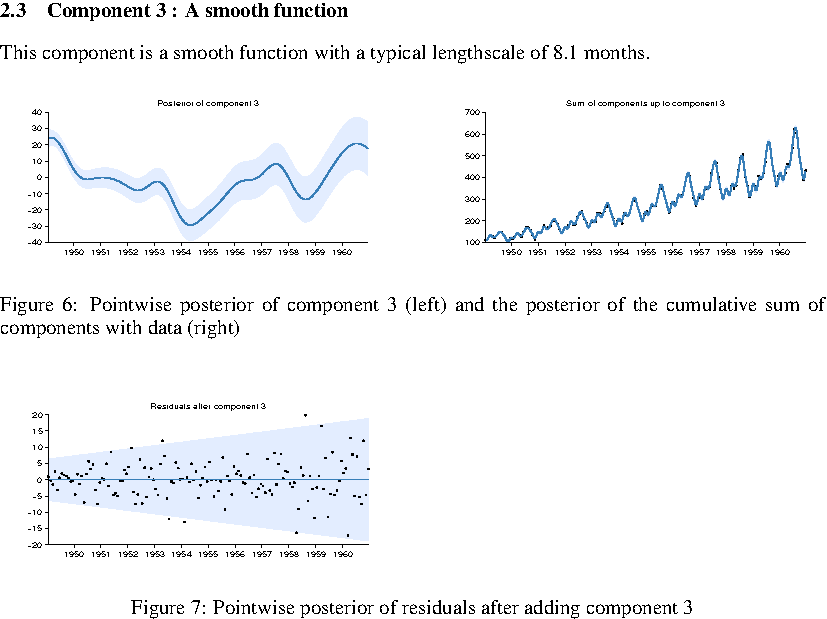
\includegraphics[trim=0cm 10.5cm 0cm 0.7cm, clip, width=0.98\columnwidth]{\grammarfiguresdir/solarpages/pg_0005-crop} \\
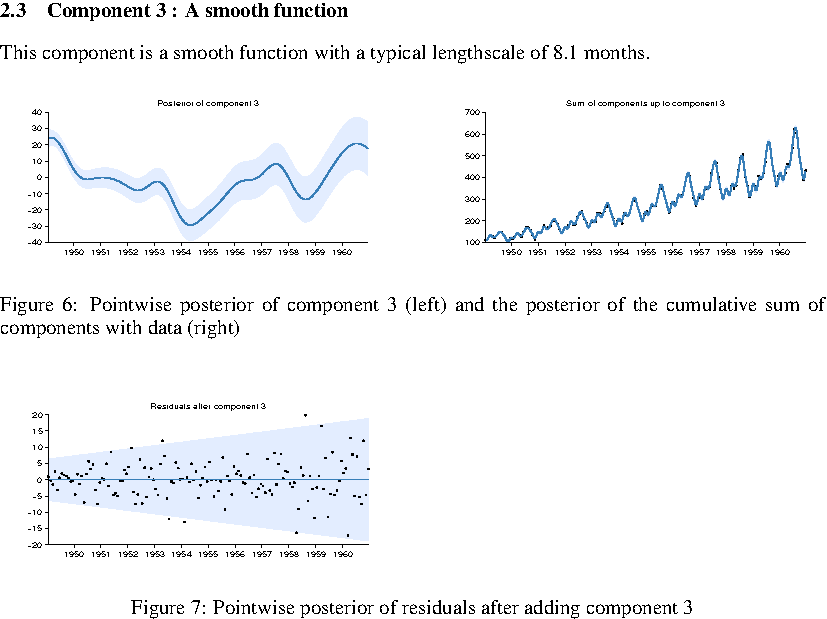
\includegraphics[trim=0cm 4.75cm 0cm 3.12cm, clip, width=0.98\columnwidth]{\grammarfiguresdir/solarpages/pg_0005-crop}
\end{tabular}
}
\caption[A component corresponding to the Maunder minimum]
{Extract from an automatically-generated report describing the model component corresponding to the Maunder minimum.}
\label{fig:maunder}
%\end{figure}
%
%\begin{figure}[h!]
\centering
\fbox{
\begin{tabular}{@{}c@{}}
\includegraphics[trim=0cm 10.5cm 0cm 1.05cm, clip, width=0.98\columnwidth]{\grammarfiguresdir/solarpages/pg_0006-crop} \\
\includegraphics[trim=0cm 4.75cm 0cm 3.9cm, clip, width=0.98\columnwidth]{\grammarfiguresdir/solarpages/pg_0006-crop}
\end{tabular}
}
\caption[\procedurename{} isolating part of the signal explained by a slowly-varying trend]
{Characterizing the medium-term smoothness of solar activity levels.
By allowing other components to explain the periodicity, noise, and the Maunder minimum, \procedurename{} can isolate the part of the signal best explained by a slowly-varying trend.}
\label{fig:smooth}
%\end{figure}
%
%\begin{figure}[ht!]
\centering
\fbox{
\begin{tabular}{@{}c@{}}
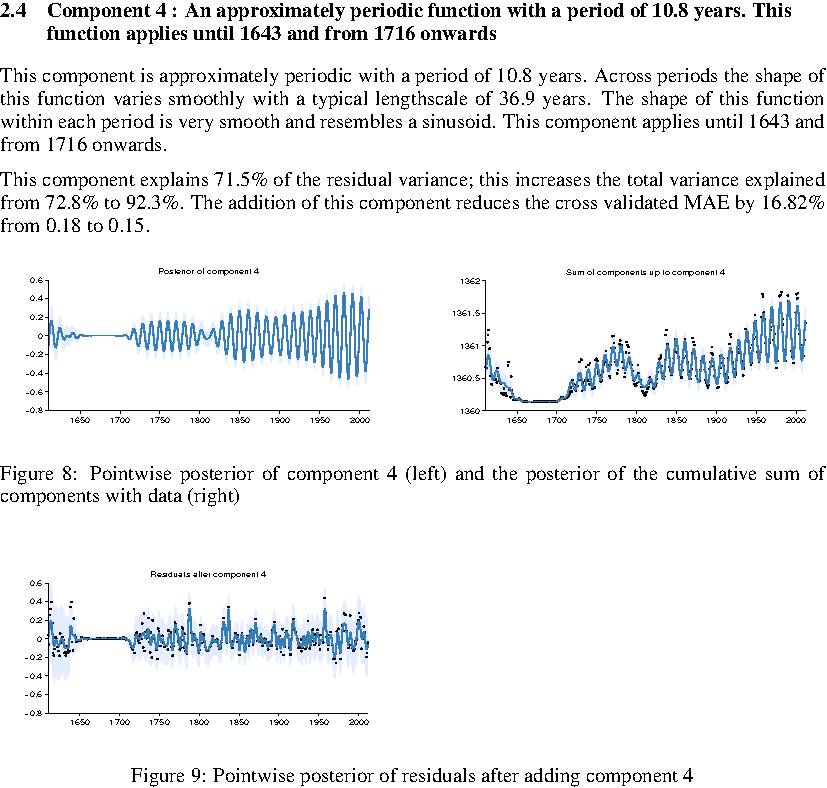
\includegraphics[trim=0cm 10.5cm 0cm 1.05cm, clip, width=0.98\columnwidth]{\grammarfiguresdir/solarpages/pg_0007-crop} \\
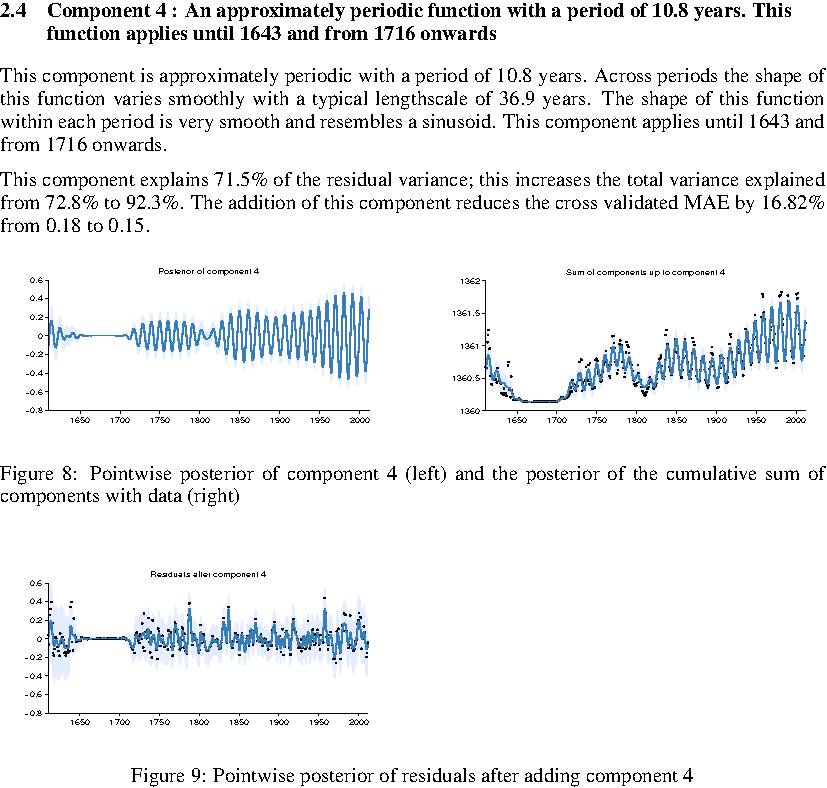
\includegraphics[trim=0cm 4.75cm 0cm 4.66cm, clip, width=0.98\columnwidth]{\grammarfiguresdir/solarpages/pg_0007-crop}
\end{tabular}
}
\caption[Automatic description of the solar cycle]
{
This part of the report isolates and describes the approximately 11-year sunspot cycle, also noting its disappearance during the Maunder minimum.}
% also noting its disappearance during the 16th century, a time known as the Maunder minimum \citep{lean1995reconstruction}.}
\label{fig:periodic}
\end{figure}
%
The complete report generated on this dataset can be found in appendix~\ref{ch:example-solar}.
Each report also contains samples from the model posterior.

\phantom{a}

%\newpage

\subsection{Describing changing noise levels} % in Air Traffic Data}
\label{sec:airline}

%\begin{figure}[ht!]
%\centering
%\includegraphics[trim=0.4cm 16.8cm 8cm 2cm, clip, width=0.5\columnwidth]{\grammarfiguresdir/airlinepages/pg_0002-crop}
%\caption[International airline passenger monthly volume dataset]
%{International airline passenger monthly volume \citep[e.g.][]{box2013time}.}
%\label{fig:airline}
%\end{figure}

Next, we present excerpts of the description generated by our procedure on a model of international airline passenger counts over time, shown in \cref{fig:airline_decomp}.
%The model described is the same as that shown in \cref{fig:airline_decomp}.
%constructed by \procedurename{} has four components: $\kLin \kernplus \kSE \kerntimes \kPer \kerntimes \kLin \kernplus \kSE \kernplus \kWN \kerntimes \kLin$, with 
%
High-level descriptions of the four components discovered are shown in \cref{fig:exec-airline}.

\begin{figure}[ht!]
\centering
\fbox{\includegraphics[trim=0cm 9.5cm 0cm 9.25cm, clip, width=0.98\columnwidth]{\grammarfiguresdir/airlinepages/pg_0002-crop}}
\caption[Short descriptions of the four components of the airline model]
{Short descriptions of the four components of a model describing the airline dataset.}
\label{fig:exec-airline}
\end{figure}

\begin{figure}[ht!]
\centering
\fbox{
\begin{tabular}{@{}c@{}}
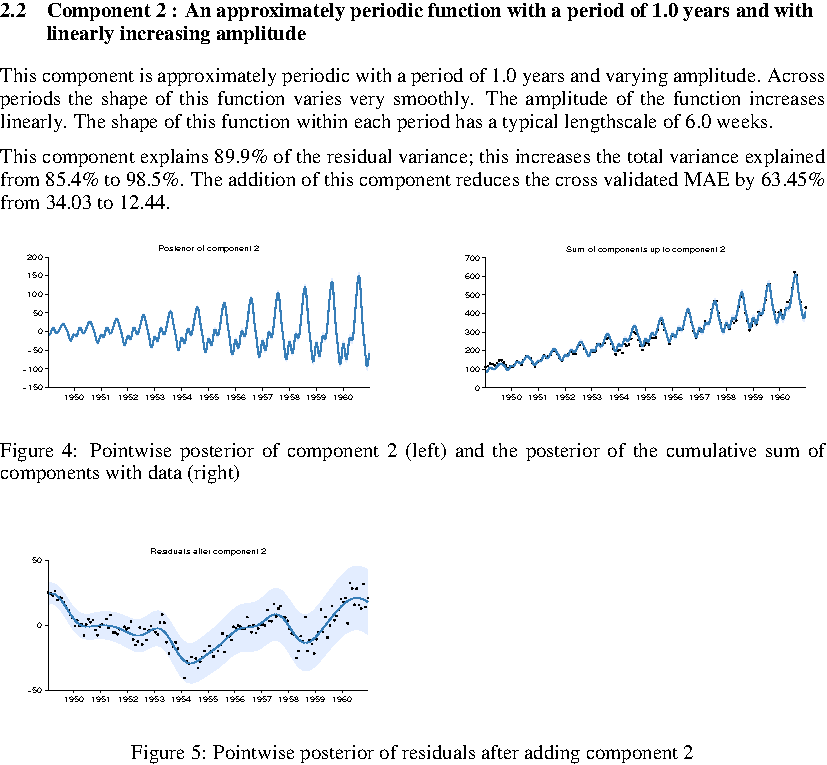
\includegraphics[trim=0cm 10.5cm 0cm 1cm, clip, width=0.98\columnwidth]{\grammarfiguresdir/airlinepages/pg_0004-crop} \\
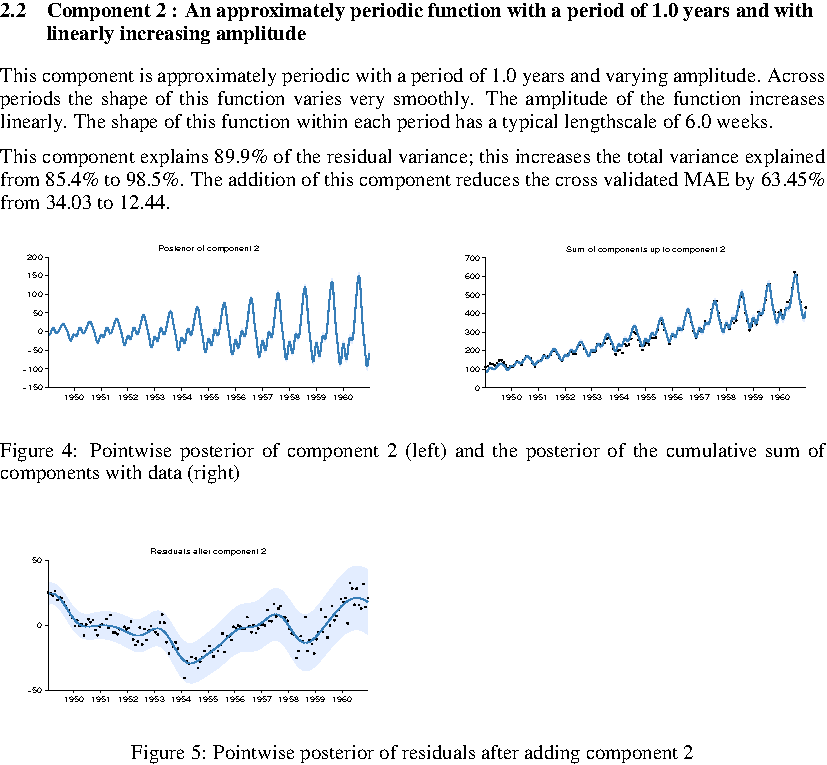
\includegraphics[trim=0cm 4.7cm 0cm 4.3cm, clip, width=0.98\columnwidth]{\grammarfiguresdir/airlinepages/pg_0004-crop}
\end{tabular}
}
\caption[Describing non-stationary periodicity in the airline data]
{Describing non-stationary periodicity in the airline data.}
\label{fig:lin_periodic}
\end{figure}

\begin{figure}[ht!]
\centering
\fbox{
\begin{tabular}{@{}c@{}}
\includegraphics[trim=0cm 6.7cm 0cm 0.6cm, clip, width=0.98\columnwidth]{\grammarfiguresdir/airlinepages/pg_0006-crop} \\
\includegraphics[trim=0cm 0cm 0cm 3.98cm, clip, width=0.98\columnwidth]{\grammarfiguresdir/airlinepages/pg_0006-crop}
\end{tabular}
}
\caption[Describing time-changing variance in the airline dataset]
{Describing time-changing variance in the airline dataset.}
\label{fig:heteroscedastic}
\end{figure}

The second component, shown in \cref{fig:lin_periodic}, is accurately described as approximately ($\kSE$) periodic ($\kPer$) with linearly growing amplitude ($\kLin$).

The description of the fourth component, shown in \cref{fig:heteroscedastic}, expresses the fact that the scale of the unstructured noise in the model grows linearly with time.
%By multiplying a white noise kernel by a linear kernel, the model is able to express heteroscedasticity (covariance which changes over time).

The complete report generated on this dataset can be found in the supplementary material of \citet{LloDuvGroetal14}.
Other example reports describing a wide variety of time-series can be found at \url{http://mlg.eng.cam.ac.uk/lloyd/abcdoutput/}


\section{Related work}
\label{sec:description-related-work}
To the best of our knowledge, our procedure is the first example of automatic textual description of a nonparametric statistical model.
However, systems with natural language output have been developed for automatic video description \citep{barbu2012video} and automated theorem proving \citep{ganesalingam2013fully}.

Although not a description procedure, \citet{durrande2013gaussian} developed an analytic method for decomposing \gp{} posteriors into entirely periodic and entirely non-periodic parts, even when using non-periodic kernels.



\section{Limitations of this approach}
\label{sec:limitations-of-abcd}

During development, we noted several difficulties with this overall approach:

\begin{itemize}

\item {\bf Some kernels are hard to describe.}
For instance, we did not include the $\kRQ$ kernel in the text-generation procedure.
This was done for several reasons.
First, the $\kRQ$ kernel can be equivalently expressed as a scale mixture of $\kSE$ kernels, making it redundant in principle.
Second, it was difficult to think of a clear and concise description for effect of the hyperparameter that controls the heaviness of the tails of the $\kRQ$ kernel.
Third, a product of two $\kRQ$ kernels does not give another $\kRQ$ kernel, which raises the question of how to concisely describe products of $\kRQ$ kernels.

\item {\bf Reliance on additivity.}
Much of the modularity of the description procedure is due to the additive decomposition.
%However, some types of structure do not allow additive decomposition.
%For example, A multiplication of , or only decompose additively after being warped.
However, additivity is lost under any nonlinear transformation of the output.
Such warpings can be learned~\citep{snelson2004warped}, but descriptions of transformations of the data may not be as clear to the end user.

\item {\bf Difficulty of expressing uncertainty.}
A natural extension to the model search procedure would be to report a posterior distribution on structures and kernel parameters, rather than point estimates.
Describing uncertainty about the hyperparameters of a particular structure may be feasible,
but describing even a few most-probable structures might result in excessively long reports.

\end{itemize}


\subsubsection{Source code}
Source code to perform all experiments is available at \\\url{http://www.github.com/jamesrobertlloyd/gpss-research}. 




\section{Conclusions}
This chapter presented a system which automatically generates detailed reports describing statistical structure captured by a \gp{} model.
The properties of \gp{}s and the kernels being used allow a modular description, avoiding an exponential blowup in the number of special cases that need to be considered.

Combining this procedure with the model search of \cref{ch:grammar} gives a system combining all the elements of an automatic statistician listed in \cref{sec:ingredients}:
an open-ended language of models, a method to search through model space, a model comparison procedure, and a model description procedure.
Each particular element used in the system presented here is merely a proof-of-concept.
However, even this simple prototype demonstrated the ability to discover and describe a variety of patterns in time series.

%We hope that systems such as these will allow the use of






\outbpdocument{
\bibliographystyle{plainnat}
\bibliography{references.bib}
}


